% !TeX root = ../main.tex

\xchapter{软硬件基础理论与前置技术}{Preliminaries}

绪论指出多核NPU面临存储墙、通信墙与编译调度墙的耦合挑战，并提出了以端到端周期级模拟支撑架构探索与瓶颈归因的研究目标。本章介绍后续模拟器设计与实验所依赖的软硬件基础与前置技术。首先概述多核NPU的体系结构基础，建立硬件组成与数据流的直观认识。其次说明深度学习工作负载的计算与访存特征，以明确模拟器需要刻画的负载形态。然后简述周期级模拟方法论，并介绍硬件模拟平台 ZeBu 作为后文准确性验证的参考依据。接着说明本文所集成的关键工具底座 BookSim2 与 Ramulator2。最后介绍多核 NPU 编译与调度的挑战与相关工作（含 SET、Gemini 等），以及调度器 IR 与本文模拟器的衔接。本章为第三、四章的整体架构设计与核心建模奠定基础。

\xsection{多核神经网络芯片体系结构基础}{Multi-core Neural Network Chip Architecture}

为便于后文理解模拟器所抽象的计算、存储与互连模块，本小节先给出通用 NPU 的典型结构概览，再分别介绍脉动阵列与数据流、以及片上 SRAM 与显式搬运，与本文建模的对应关系。NPU在计算、数据流与存储层次等方面的设计空间与权衡可参见综述\cite{sze2017efficient}。

在芯片级，NPU 常采用多核布局：处理单元（Processing Element, PE）阵列构成计算核心，周围分布本地缓存或输入输出缓冲，通过片外接口与主存或其他芯片互联。各计算核心之间由片上网络（NoC）连接，形成可扩展的多核拓扑。业界代表性设计如 Google TPU 采用脉动阵列与高带宽片内存储实现数据中心级推理加速\cite{jouppi2017tpu}，NVDLA 等开源架构则提供了可配置的卷积与数据处理器模块，便于软硬件协同评估\cite{veronesi2021nvdla}。多核扩展在提升峰值算力的同时，也使得核间数据搬运与共享存储访问成为系统级瓶颈。NoC 的拓扑与路由、以及各核与片外存储的带宽分配，共同决定了实际可达的利用率和尾延迟。在单核或单簇内部，典型功能模块包括：控制单元负责指令或调度序列的解析与下发。数据传输单元包含 DMA 与 NoC 路由器，负责片内与片外数据的搬运及与邻核的通信。全局缓存（或层次化 SRAM）作为输入特征图、权重与输出特征图的暂存与共享区。处理单元阵列（如脉动阵列）执行矩阵乘、卷积等 MAC 密集运算。向量处理单元则负责激活、归一化等逐元素或向量运算。数据在“全局缓存 $\leftrightarrow$ 处理单元阵列 $\leftrightarrow$ 向量处理单元”以及“数据传输单元 $\leftrightarrow$ 片外DRAM”之间按调度流动。图\ref{fig:c2_npu_generic}给出上述通用结构的示意，便于读者建立对 NPU 组成与数据流的大致认识。左半部分是芯片级多核布局（处理单元、本地缓存/输入输出、片外接口及互连），右半部分描述了单核/簇内部功能模块与数据流（控制单元、数据传输单元、全局缓存、处理单元阵列、向量处理单元及输入特征图/权重/输出特征图流向）。如绪论所述，Cerebras 等晶圆级设计将多核扩展推向极致。本文模拟器对“处理单元阵列”抽象为可配置的乘加器数目与向量单元数目，对“全局缓存/本地 SRAM”抽象为容量与生命周期约束，对“数据传输单元”中的 NoC 与片外接口则通过网络接口与存储接口对接，详见第三、四章。

\begin{figure}[htbp]
  \centering
  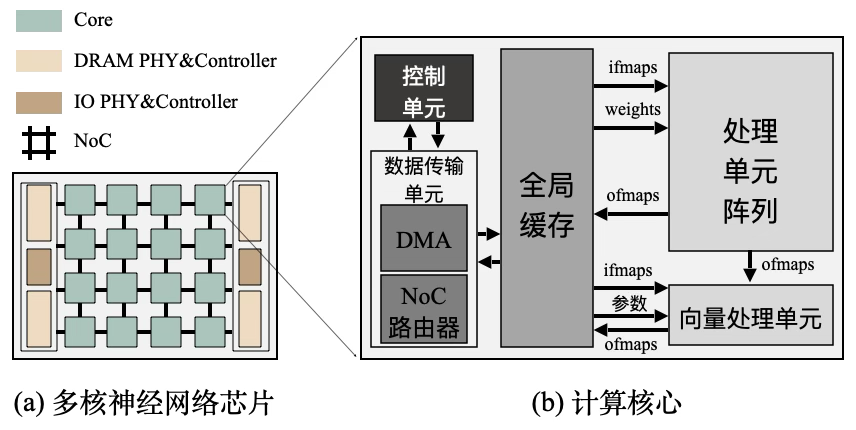
\includegraphics[width=0.95\textwidth]{Figures/npu_generic_arch.png}
  \caption{一种通用 NPU 的典型结构示意图}
  \label{fig:c2_npu_generic}
\end{figure}

\xsubsection{脉动阵列与数据流}{Systolic Array and Dataflow}

脉动阵列通过规则的数据流与邻近通信实现高数据复用，是 NPU 中常见的核心计算结构。数据在阵列内按“脉动”节奏流动，同一数据在多个 PE 间复用，从而降低对片外带宽的依赖。不同数据流策略（如权重驻留、输出驻留、行驻留等）会改变权重与激活在阵列上的驻留方式，进而影响片上 SRAM 占用、核间/核外数据搬运量以及 DRAM 访问模式，从而在系统层面表现为不同的计算—通信—存储平衡。图\ref{fig:c2_dataflow}展示了多核 NPU 架构下的片上数据流示意。张量数据通过片外 DRAM 加载至片上网络（NoC），在不同计算核心的 SRAM 之间进行传输与复用，完成计算后再将最终结果写回 DRAM。这种显式的数据搬运与通信机制显著降低了对片外带宽的依赖。Eyeriss 等工作系统刻画了行驻留等数据流对能效与复用率的影响\cite{chen2016eyeriss}。MAESTRO 则以数据为中心对 DNN 映射的复用、性能与硬件代价进行快速解析建模，为设计空间探索提供了工具基础\cite{kwon2019maestro}。本文关注多核系统级瓶颈与设计空间探索。模拟器对单核计算采用“可参数化的乘加器数目与向量单元数目等吞吐能力 + 显式数据搬运依赖”的抽象，不展开阵列内部数据流细节。实验中可通过调节计算资源参数与映射方式，间接体现数据流与映射对端到端性能的影响。

\begin{figure}[htbp]
  \centering
  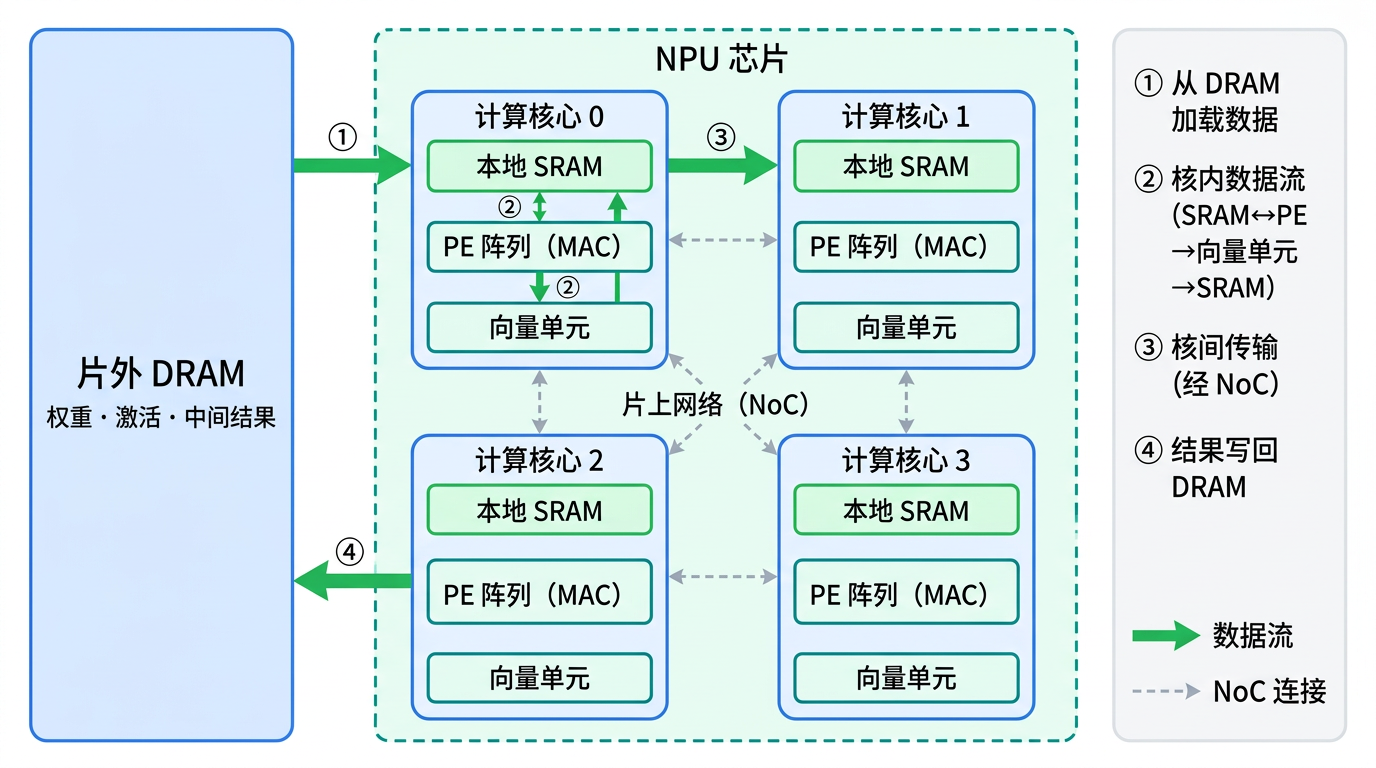
\includegraphics[width=0.98\textwidth]{Figures/c2_dataflow_v12.png}
  \caption{多核 NPU 片上数据流示意图}
  \label{fig:c2_dataflow}
\end{figure}

在微架构层面，脉动阵列内部的数据流可进一步细化。图\ref{fig:c2_systolic}给出了一个 3$\times$3 脉动阵列的数据流示意。权重沿水平方向逐拍向右传递（绿色箭头），激活沿垂直方向逐拍向下传递（蓝色箭头），每个 PE 在每拍接收来自左侧的权重与上方的激活，执行一次乘加（MAC）操作后将数据传递给相邻 PE。部分和在阵列右侧输出。这种规则的数据流动使得每份数据在多个 PE 间被复用，从而以较低的片外带宽需求实现高吞吐的矩阵运算。

\begin{figure}[htbp]
  \centering
  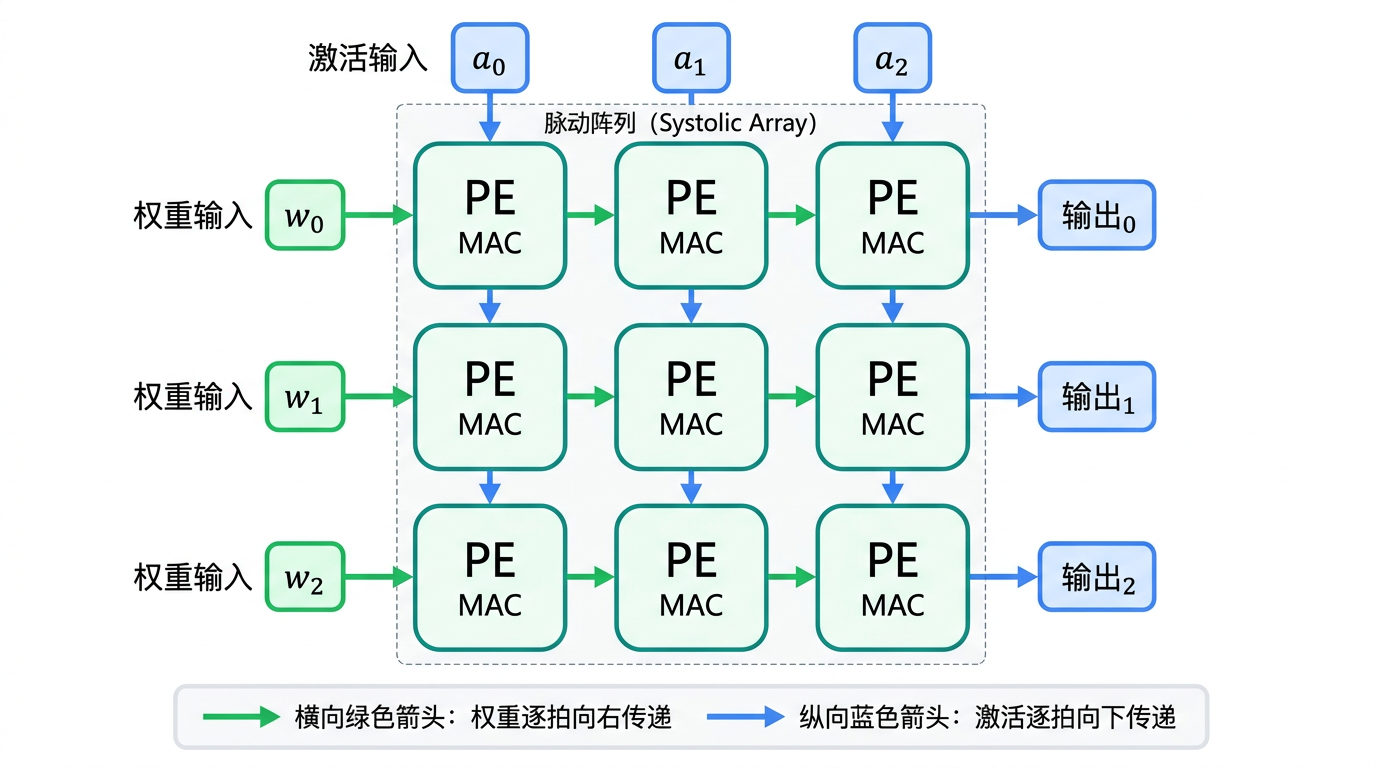
\includegraphics[width=0.85\textwidth]{Figures/c2_systolic_array_v2.png}
  \caption{3$\times$3 脉动阵列数据流示意图}
  \label{fig:c2_systolic}
\end{figure}

\xsubsection{片上SRAM与显式搬运}{Scratchpad SRAM and Explicit Data Movement}

与传统 CPU 的缓存不同，NPU 常采用编译器或调度器显式管理的片上缓存（常用 SRAM/TCM 构成）。编译与调度在空间上把张量切分为小块，在时间上决定何时搬运、何时计算以及搬运与计算的重叠程度。双缓冲等技术可在计算当前块的同时预取下一块，从而提高计算单元利用率。片上容量、端口带宽与数据驻留生命周期共同决定了可选的分块粒度与复用效率，也是多核系统中“存储墙”形成与缓解的关键因素\cite{reuther2024memorywall}。 本文模拟器对每核配置本地 SRAM 容量，并通过传输标识与引用计数刻画多消费者共享同一输出时的驻留需求，从而在周期级推进中反映 SRAM 约束对可行映射与端到端周期的影响。

\xsection{深度学习工作负载的计算与访存特征}{Workload Characteristics}

在明确 NPU 的典型结构与存储、互连层次之后，本小节在人工智能与大模型发展的背景下，简要总结运行于 NPU 上的深度学习工作负载的计算与访存特征，以便理解模拟器所需刻画的负载形态及其对架构与调度的要求。

\textbf{人工智能与大模型发展对 NPU 的需求背景。} 近年来，以深度学习为代表的人工智能技术在计算机视觉、自然语言处理、多模态理解等任务上取得显著进展，模型规模与数据量持续增长，对算力与能效提出了更高要求\cite{hennessy2019golden}。基于 Transformer 架构的大规模预训练模型（大模型）在自然语言理解与生成、代码生成、逻辑推理等场景中成为主流形态，参数规模从数亿至数万亿不等。云端与边缘侧的部署与推理需求推动了专用加速器与多核 NPU 的发展\cite{zhao2023llm_survey}。模型演进、训练算力需求与 NPU 性能代际提升之间的呼应关系已在第一章绪论图\ref{fig:c1_npu_performance_timeline} 与图\ref{fig:c1_dl_training_compute} 中概括给出（其中图\ref{fig:c1_dl_training_compute} 刻画训练算力随年份的指数增长趋势\cite{sastry2024computing}）。大模型在训练与推理阶段均表现出强烈的计算密集与访存密集特征。随序列长度、批次大小与模型深度的变化，计算与存储、通信的瓶颈会发生转移，这对周期级模拟与多核调度评估提出了明确需求。因此，将深度学习与大模型负载的特征纳入前置知识，便于后文理解模拟器刻画的层间依赖、数据量与阶段划分同真实负载的对应关系。

\textbf{算子与模型形态的多样性。} 深度学习模型可视为由张量算子构成的计算图，不同算子在算术强度、访存形态与可融合性上差异显著。卷积神经网络（Convolutional Neural Network, CNN）类模型以卷积与全连接（GEMM）为主，计算图相对规整，层间数据量可预测。Transformer 类模型则引入自注意力、层归一化等算子，访存模式与序列长度和批次大小强相关。量化等方法在保证精度的前提下降低访存与计算量，是部署阶段常用的优化手段\cite{ding2020survey}。GEMM、卷积等 MAC 密集算子计算量大、访存相对集中，在充足算力与带宽供给下更容易接近峰值吞吐。归约、归一化、激活与逐元素算子则往往带宽受限，其性能对片上和片外内存带宽更为敏感。批量大小、序列长度与特征维度等参数直接决定每层的张量体积与访存量。多核映射时需在算力均衡与数据搬运代价之间折中。多核 NPU 模拟器需要能够区分这类差异，以便在周期级模型中合理分配计算周期与访存延迟。

\textbf{大模型推理与注意力、KV Cache 的访存特征。} 以 Transformer 为代表的基础模型在云端与端侧被广泛部署，其自注意力机制具有显著的长序列与 KV Cache 特征。朴素自注意力的计算与存储复杂度随序列长度 $L$ 呈 $O(L^2)$ 增长，在长序列场景下输入输出与带宽成为主要瓶颈。FlashAttention 等工作通过分块计算与重计算权衡降低了片外访存与带宽压力\cite{vaswani2017attention,dao2022flashattention,dao2023flashattention2}。在大模型推理服务中，KV Cache 的容量与访问模式对内存碎片与带宽利用率影响巨大，PagedAttention 及 vLLM 等通过分页式 KV Cache 管理显著提升了吞吐\cite{kwon2023pagedattention}。本文模拟器以调度器 IR 为输入，不直接建模算子内部实现。但所承载的 ResNet、Transformer 等负载的层间依赖与数据量特征，仍将反映上述计算与访存特性在端到端周期上的影响。后文实验采用的 ResNet 系列负载兼具卷积与全连接等典型算子，便于观察计算与访存在不同阶段的占比。其结论在方法论上对面向大模型的多核 NPU 评估具有参考价值。

\xsection{周期级模拟方法与系统级建模}{Cycle-level Simulation}

从模拟范式看，踪迹驱动方法以离线生成的执行踪迹回放为主，执行闭环较弱，难以自然反映因资源争用与反压导致的时序变化。执行驱动方法则以任务或指令驱动系统推进，能够体现排队、背压与依赖满足的连锁效应，更适合多核 NPU 的端到端分析与瓶颈归因\cite{zhang2023gem5nvdla}。 本文采用执行驱动的周期级模拟。模拟器按全局周期步进，每一拍可更新核心状态、NoC 报文与 DRAM 请求的进展，事件顺序与资源占用在时间轴上一致，从而在保证因果正确的前提下得到可重复的周期估计。以调度器输出的工作负载与依赖为驱动，在统一时间轴上推进各核心与 NoC、DRAM，使“依赖到齐—计算—写回”的因果与竞争行为在模拟中可复现。周期级精度意味着每个全局周期内各子系统的状态更新与事件顺序可被显式建模，从而能够捕捉 NoC 拥塞、DRAM 行缓冲冲突等对端到端延迟的非线性影响，为设计空间探索提供可信的定量依据。近期多核 NPU 模拟器（如 ONNXim）也强调对 NoC 与 DRAM 竞争的建模，以提升系统级瓶颈刻画能力\cite{jin2024onnxim}，与本文思路一致。

\xsection{硬件模拟与准确性验证参考：ZeBu}{Hardware Emulation and ZeBu as Validation Reference}

周期级模拟器的结果是否可信，需要与更接近真实硬件的参考进行对比。除流片实测外，基于硬件模拟的原型验证是常用参考手段。将 RTL 综合并部署到硬件模拟平台（如基于现场可编程门阵列（Field-Programmable Gate Array, FPGA）或专用模拟机的原型系统），在接近真实时钟与时序约束下运行，得到指令级或周期级的执行踪迹，可作为“金标准”用于校验模拟器的周期估计。

ZeBu 是业界常用的硬件模拟平台之一，能够将 NPU 等设计的 RTL 在模拟环境中运行，并输出每条指令的执行时间区间（即起始周期与结束周期）。在相同调度配置与相同输入 IR 的前提下，ZeBu 运行得到的踪迹可汇总为总执行周期（即各指令结束周期的最大值），与本文模拟器在相同 IR、相同核心数等配置下得到的端到端总周期进行对比。若二者相对误差在可接受范围内（如 5\%--15\%），则可为模拟器的准确性提供佐证。实践中常采用单核或与 ZeBu 相同的核心数配置进行对比，以保证调度与数据流一致、便于归因差异。本文第五章在开展微基准与真实负载实验时，将视需要引入 ZeBu 踪迹与模拟器结果的对比，以说明模拟器在周期级行为上与参考实现的一致性。本节对 ZeBu 的角色与定位做预先说明，为第五章中与 ZeBu 的对比实验提供背景。

\xsection{关键工具底座：BookSim2与Ramulator2}{BookSim2 and Ramulator2}

本文模拟器在“高保真”模式下将片上网络与片外存储分别委托给 BookSim2 与 Ramulator2，以复用其成熟的周期级建模能力。本节简要说明二者在本文中的角色，为第三、四章的接口设计与集成提供依据。

\xsubsection{BookSim2：周期级NoC模拟}{BookSim2 for NoC}

BookSim（及其后续版本 BookSim2）提供可配置的周期级 NoC 模拟，支持多种拓扑（如 Mesh、Torus）、路由算法（如 XY、自适应路由）、虚拟通道（VC）数量与缓冲深度、以及分片与数据包的划分\cite{jiang2013booksim}。 Mesh 等规整拓扑便于随核心数扩展且路由规则简单。虚拟通道在同一物理链路上提供多条逻辑通道，有助于缓解队头阻塞、提升吞吐。模拟按周期推进，每周期内完成路由计算、VC 分配、交换仲裁与链路传输，从而能够刻画多流并发时的排队与背压。通过配置拓扑与路由，可研究拥塞、仲裁与尾延迟对端到端性能的影响。本文通过封装 BookSim2 作为片上网络接口的一种实现，在保持与执行层解耦的前提下，将多核产生的核间读请求与响应映射为 NoC 上的数据包流，并接收其周期级投递结果以驱动依赖满足与状态推进。

\xsubsection{Ramulator2：DRAM时序与调度}{Ramulator2 for DRAM}

主存方面，DRAM 的时序约束（如 $t_\mathrm{RCD}$、$t_\mathrm{RP}$、$t_\mathrm{RAS}$）、Bank 并行度与调度策略（如 FR-FCFS）对有效带宽影响显著。其中 $t_\mathrm{RCD}$ 为行激活延迟，$t_\mathrm{RP}$ 为预充电时间，$t_\mathrm{RAS}$ 为行有效至预充电的最短间隔。行缓冲命中可大幅缩短访问延迟，而 Bank 冲突与行关闭则引入额外周期。多核并发时排队与调度顺序会显著改变实际带宽利用率。Ramulator2 以模块化、可扩展的方式实现了多种 DRAM 标准（如 DDR4）的时序与调度建模，支持通道数、Bank 组织、行缓冲与刷新等配置，便于研究排队、行命中与冲突对多核并发访存的影响\cite{luo2023ramulator2}。 本文通过封装 Ramulator2 作为片外存储接口的一种实现，将核心发起的读写请求注入 Ramulator2，并按模拟器配置的存储与核心时钟比进行多速率推进，使 DRAM 行为与核心/NoC 时间轴对齐，支撑端到端周期与存储瓶颈分析。

\xsection{多核神经网络芯片编译与调度及调度器IR}{Compilation, Scheduling, and Scheduler IR}

\xsubsection{编译与调度的挑战与相关工作}{Challenges and Related Work}

在多核 NPU 上，将深度神经网络（DNN）工作负载映射到各计算核心并确定层间/算子间的执行顺序与数据放置，是编译与调度的核心问题。不同映射与调度策略会导致数量级级的性能与能效差异。

在编译与中间表示方面，TVM 等端到端优化编译器通过图级与算子级优化、学习式代价模型与多后端支持，实现了从高层模型到 FPGA、专用集成电路（Application-Specific Integrated Circuit, ASIC）等多种加速器的性能可移植\cite{chen2018tvm}。MLIR 等多层中间表示基础设施为领域专用后端提供了可扩展的抽象与变换管道，便于从高层图表示下译到硬件相关指令\cite{lattner2021mlir}。面向具体 NPU 的编译栈（如 Hexagon-MLIR）在此基础上实现了从模型到 NPU 指令的完整链路\cite{qualcomm2026hexagonmlir}。在架构与映射评估方面，Timeloop 对 DNN 加速器的工作负载映射与性能评估提供了系统化方法，Accelergy 则从架构级对能效进行估计，二者常配合用于设计空间探索\cite{parashar2019timeloop,wu2019accelergy}。MAESTRO 以数据为中心刻画 DNN 数据流与映射的复用、延迟与能耗，为快速解析评估提供了工具\cite{kwon2019maestro}。

在层间与多核调度方面，SET\cite{set2023isca} 针对分片式加速器，对层间调度空间进行了形式化定义与系统探索，为各层计算资源的分配与执行顺序提供了可操作的搜索空间，避免了仅依赖启发式规则带来的次优解。Gemini\cite{cai2024gemini} 则面向多核架构，提出层流水空间映射编码，并结合图划分与模拟退火进行映射与架构的协同探索，其输出的调度方案以结构化 IR 形式描述，可直接驱动硬件模拟或周期级模拟器执行。图\ref{fig:c2_mapping}给出了多核架构下典型的工作负载映射示意。模型各层被分配至不同的计算核心，通过核间通信实现层间流水与空间并行，从而最大化硬件利用率并降低端到端延迟。Tetris 等工作则从 3D 堆叠存储与数据放置角度探讨了可扩展的神经网络加速与带宽利用\cite{gao2017tetris}。上述工作分别从编译基础设施、架构—映射评估与层间/多核调度等角度，为多核 NPU 的编译调度与本文所采用的调度器 IR 提供了理论与工具基础。

\begin{figure}[htbp]
  \centering
  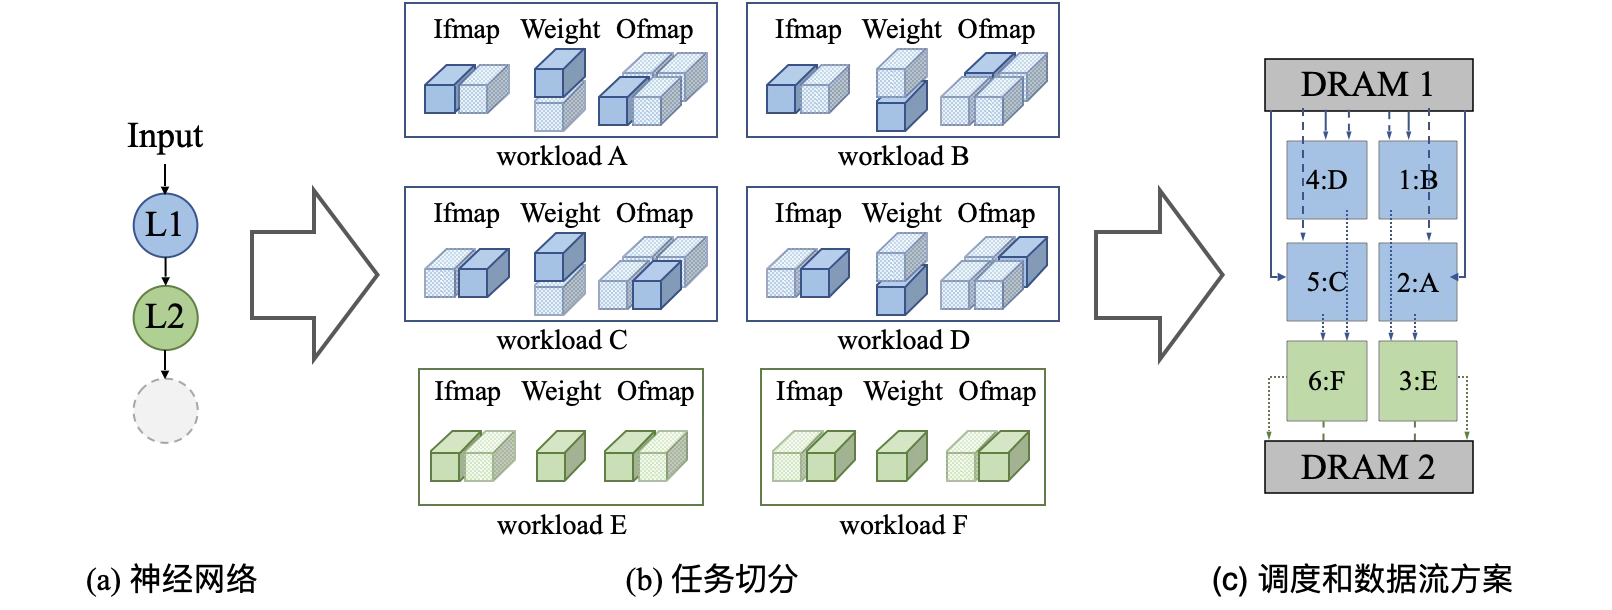
\includegraphics[width=0.9\textwidth]{Figures/mapping.png}
  \caption{多核 NPU 上的层间流水与空间映射示意图}
  \label{fig:c2_mapping}
\end{figure}

\xsubsection{调度器如何生成IR及IR的形式与语义}{How the Scheduler Produces IR and IR Specification}

本模拟器以 Gemini 调度器（开源框架见 \url{https://github.com/SET-Scheduling-Project/GEMINI-HPCA2024}）输出的 IR 为工作输入，因此有必要明确 IR 的来源、生成过程及其应包含的信息与语义。

\textbf{IR 的来源与生成过程。} 调度器在完成层间/层内映射与执行顺序搜索后，将结果编码为结构化 IR 并写出为 JSON 文件。以 Gemini\cite{cai2024gemini} 为例：在给定核心网格与 SRAM 等约束下，通过层流水空间映射编码与模拟退火等搜索得到“每一层（或算子组）分配到哪些核心、以何种顺序执行、数据从何而来、写往何处”。随后将这些决策转化为 IR 中的核心网格规模、每核上的工作负载列表，以及各工作负载的输入依赖与输出描述。因此，IR 本质上是“映射与调度结果”的可执行表示。模拟器或硬件后端只需按 IR 中的依赖与数据量推进，无需再做映射决策。

\textbf{IR 应包含的内容与语义。} 为驱动周期级模拟，IR 至少需表达以下几类信息。（1）核心网格与全局约束：如核心数量（或 $x\times y$ 网格）、可选的全局 SRAM 容量上限等，用于约束资源与规模。（2）每核工作负载序列：每个核心对应一个工作负载列表，列表中的每一项表示“在该核上执行的一个计算单元”，通常对应某一层或某一算子在某一数据分片上的执行。每项需包含算子类型、输出张量规模（如输出特征图尺寸、权重尺寸等），以便模拟器推算计算量与访存量。（3）依赖关系：每个工作负载的输入由输入缓冲（或输入依赖）描述，每一项引用一个传输标识（或等价标识），表示该数据由哪一个生产者的哪一输出产生。模拟器据此建立“数据产生 $\leftrightarrow$ 传输/写回 $\leftrightarrow$ 被消费”的依赖链，只有依赖到齐后该工作负载才能进入计算阶段。（4）输出与消费者：每个工作负载的输出描述给出其输出对应的传输标识，供后续工作负载或 DRAM 写回引用。多消费者可共享同一传输标识，由模拟器通过引用计数或等价机制管理驻留与释放。此外，若调度器区分了来自 DRAM 的读与来自他核的读，IR 中可显式标注数据来源（如 DRAM 读入、核间读），以便模拟器分别走存储接口与 NoC 接口。综上，IR 的形式是“核心网格 + 每核工作负载列表 + 每工作负载的依赖与输出标识及数据量”。模拟器据此即可在统一周期轴下按依赖推进，发起 NoC/DRAM 请求并统计周期与瓶颈。

\xsubsection{调度器IR与本文模拟器的衔接}{Scheduler IR and Simulator Input}

由上可见，Gemini 等框架输出的调度器 IR 以 JSON 形式承载上述核心网格、每核工作负载序列、各工作负载的输入依赖与输出描述及数据量等信息。每个工作负载对应某一层（或算子）在某一核心上的执行单元，依赖关系与数据量在 IR 中显式给出，便于模拟器按“依赖满足—计算—写回”的语义推进。本文模拟器即以此类 IR 为可执行的上游输入。本小节从 Gemini 与模拟器的分工与衔接、以及 Gemini-Compiler-IR 项目所提供的基准调度 IR 与 ZeBu 踪迹在第五章实验中的使用两方面，说明调度器 IR 在本文研究中的角色与意义。

\textbf{Gemini 与本文模拟器的关系。} 从功能分工看，Gemini 负责“映射与调度”的搜索与决策。在给定核心网格、SRAM 容量等约束下，通过层流水空间映射编码与模拟退火等算法，确定每一层分配到哪些核心、以何种顺序执行、数据从何而来与写往何处，并将结果编码为结构化 JSON IR 写出。本文模拟器则不参与映射搜索，仅作为“执行后端”。它以 Gemini 输出的 IR 为工作负载输入，在统一周期轴上按依赖推进各核心的加载、计算与写回，并同时推进 NoC 与 DRAM 的请求与响应，从而得到端到端周期与瓶颈统计。二者在逻辑上形成“Gemini 生成调度 $\rightarrow$ IR 描述 $\rightarrow$ 模拟器执行并反馈周期与瓶颈”的流水线。这一分工的意义在于：调度器专注于映射空间探索与决策，模拟器专注于在给定调度下对周期级行为与瓶颈的刻画。模拟器输出的周期与阶段分解既可验证某一调度方案的实际效果，也可为后续映射搜索或架构参数设计提供定量依据，从而支撑“编译—架构”协同优化。

\textbf{Gemini-Compiler-IR 项目与 ZeBu 踪迹在本文中的作用。} Gemini-Compiler-IR 项目汇集与 Gemini/SET 工作流兼容的调度 IR，以及在同一调度下于 Synopsys ZeBu 硬件仿真平台得到的执行踪迹，被用作评估编译调度与周期级建模的参照\cite{cai2024gemini}。本文第五章的验证与瓶颈分析实验采用该项目发布的 JSON 调度文件（如 ResNet34、ResNet50 在单核、不同批大小等配置）作为模拟器输入，并采用同一批调度在 ZeBu 上测得的总周期作为对照。调度文件描述已确定的映射与依赖，ZeBu 踪迹则提供与之一致的指令级执行时间参考，二者同源，使模拟器输出可在相同调度、相同配置下与硬件仿真公平对比。本文模拟器前端将上述 JSON IR 解析为与格式无关的统一任务表示（含整体解析数据与各工作负载项），并在统一周期轴下与 NoC、DRAM 后端耦合推进，形成“调度器 IR $\leftrightarrow$ 解析 $\leftrightarrow$ 执行 $\leftrightarrow$ 统计”的链路。第三、四章将在此基础上分别介绍模拟器的整体架构与松耦合接口设计、以及可配置计算核心与全系统同步机制。
